% This is samplepaper.tex, a sample chapter demonstrating the
% LLNCS macro package for Springer Computer Science proceedings;
% Version 2.20 of 2017/10/04
%
\documentclass[runningheads]{llncs}
%
\usepackage{graphicx}
% Used for displaying a sample figure. If possible, figure files should
% be included in EPS format.
%
% If you use the hyperref package, please uncomment the following line
% to display URLs in blue roman font according to Springer's eBook style:
% \renewcommand\UrlFont{\color{blue}\rmfamily}

\begin{document}
%
\title{Chess-Num Puzzles Solver}
%
%\titlerunning{Abbreviated paper title}
% If the paper title is too long for the running head, you can set
% an abbreviated paper title here
%
\author{Diogo Samuel Gonçalves Fernandes \and
Paulo Jorge Salgado Marinho Ribeiro}
%
\authorrunning{F. Author et al.}
% First names are abbreviated in the running head.
% If there are more than two authors, 'et al.' is used.
%
\institute{Faculdade de Engenharia da Universidade do Porto, Portugal}
%Grupo e turma
%\url{$https://sigarra.up.pt/feup/pt/web_page.inicial$}
% FEUP-PLOG, Turma 3MIEIC06, Grupo Chess-Num_2
%\email{up201806250@fe.up.pt}
%\email{up201806505@fe.up.pt}
%
\maketitle              % typeset the header of the contribution
%
\begin{abstract}
Este segundo projeto da unidade curricular Programação em Lógica (PLOG) consiste na resolução de problemas
de otimização/decisão, recorrendo ao uso de restrições em Prolog. No caso do nosso grupo, o objetivo é resolver
os puzzles do tipo "Chess-Num", no menor tempo possível, com recurso a restrições, através do uso da biblioteca clpfd do SICStus Prolog.

\keywords{Programação em Lógica  \and Prolog \and Restrições \and clpfd \and SICStus \and Problemas de Otimização \and Problemas de Decisão.}
\end{abstract}

\section{Introdução}
A Programação em Lógica com Restrições trata-se de uma classe de linguagens de programação, que combina a declaratividade característica da programação em lógica
e a eficiência da resolução de restrições. As suas principais aplicações baseiam-se na resolução de problemas de pesquisa ou otimização combinatória, tal como problemas de escalonamento, geração de horários, alocação de recursos, gestão de produção, entre outros.
Dada a sua distinção e eficiência, a Programação em Lógica com Restrições tem diversas aplicações industriais e comerciais na atualidade, destacando-se a sua utilização na Renault, para planeamento de produção a curto prazo, na Nokia, para configuração de software para telemóveis, e na Siemens, para verificação de circuitos.
Neste trabalho, aplicaremos estas capacidades na resolução de puzzles Chess-Num, que consistem na colocação de uma peça de Xadrez de cada tipo (Peão, Torre, Bispo, Cavalo, Rainha, Rei) num tabuleiro com casas numeradas, de modo a que todas as casas numeradas sejam atacadas N vezes, sendo N o número apresentado nessas casas. 
Alguns exemplos de puzzles deste tipo podem ser observados aqui: https://erich-friedman.github.io/puzzle/chessnum/
Este relatório procura explicar a nossa abordagem do problema de forma aprofundada e organizada nos seguintes tópicos:

 - Descrição do Problema, com explicação de todas as regras a cumprir
 - Abordagem, onde explicaremos a nossa implementação do problema, com enumeração das variáveis de decisão e dos seus domínios
 - Visualização da Solução, com exploração dos predicados que permitem a visualização do problema resolvido, e respetivas imagens exemplificativas
 - Experiências e Resultados, onde faremos a análise dimensional do problema, para distintas quantidades de células numeradas, e  
 - Conclusões e Trabalho Futuro, onde iremos debater as principais conclusões que retiramos deste projeto, com base nos resultados obtidos, e sugerir formas de melhorar o trabalho desenvolvido
 - Referências, com enumeração das várias fontes bibliográficas que utilizamos para a procura de conhecimento
 - Anexos, que contêm imagens explicativas de alguma secção do relatório, e imagens exemplificativas do programa em execução

\section{Descrição do Problema}
Um Puzzle envolvendo peças de xadrez. No tabuleiro vão existir casas numeradas. Cada uma destas casas vai ter de estar
a ser atacada por cada uma das seis peças distintas existentes num tabuleiro de xadrez (Peão, Torre, Bispo, Cavalo, Rainha, Rei). As peças atacam como num jogo de xadrez normal.
O peão ataca para cima e para o lado, o cavalo ataca em L, o bispo ataca todas as diagonais, a torre todas as verticais e horizontais. O rei ataca todas as casas à sua volta e a 
rainha todas as diagonais, verticais e horizontais. É importante referir ainda que ao contrário do jogo de xadres é possível colocar os peões 
na primeira e última linha. Não é possível colocar duas peças
 no mesmo quadrado, nem num quadrado que tenha numeração.

 
\section{Abordagem ao Problema}
Descrever a modelação do problema como um PSR / Portugal

\subsection{Variáveis de Decisão}
    - PawnX
    - PawnY
    - KnightX
    - KnightY
    - KingX
    - KingY
    - RookX
    - RookY
    - BishopX
    - BishopY
    - QueenX
    - QueenY

    Estas variáveis de decisão são reunidas numa lista, Positions, que será depois utilizada ao efetuar o labeling.
    Cada par destas variáveis corresponde à posição de uma dada peça no tabuleiro, sendo o primeiro elemento do par a linha onde a peça se encontra, e o segundo elemento a coluna.
    Assim, as variáveis pertencem ao domínio [1, 8], que são os valores possíveis que a linha/coluna pode tomar num tabuleiro de Xadrez (8x8).
    
\subsection{Restrições}

\section{Visualização da Solução}

Para uma melhor compreensão das soluções encontradas, decidimos implementar duas formas de apresentação das soluções:
 - Forma Escrita:
    Apresenta-se no ecrã as posições de cada uma das seis peças, no formato [Linha, Coluna].
    Isto é efetuado pelo predicado show\textunderscore results, que recebe a lista das posições das peças e o número da peça a que a próxima posição corresponde. Trata-se de um ciclo simples, e recorre ao predicado piece, que recebe o número da peça e retorna o respetivo nome.
    Tanto a implementacão deste predicado como o seu funcionamento com o programa em execução podem ser visualizados nos anexos. (LINK IMAGENS)
 - Tabuleiro:
    É apresentado um tabuleiro com as células numeradas e com as seis peças já colocadas conforme a solução encontrada.
    Isto é efetuado pelo predicado display\textunderscore solution, que chama o predicado add\textunderscore pieces, responsável por substituir os valores das células dos tabuleiros contidos em Positions, pela peça de Xadrez correspondente. De seguida, é chamado o predicado display\textunderscore board, que representa visualmente o tabuleiro já preenchido.
    Da mesma forma, é apresentado o tabuleiro do problema (apenas com as células numeradas) antes de se iniciar a procura da solução.

\section{Experiências e Resultados}
\subsection{Análise Dimensional}
Quantas mais casas numeradas existirem, mais lento é o programa
\subsection{Estratégias de Pesquisa}

\section{Conclusões e Trabalho Futuro}

A realização deste trabalho permitiu a resolução de um problema através da utilização de restições lógicas na linguagem PROLOG, através da utilização do módulo CLPFD.
Durante a realização do mesmo foram encontradas diversas dificuldades, nomeadamente na elaboração dos ataques para a torre a para o bispo, uma vez que se existir alguma peça no seu caminho esta só ataca até essa peça.

O tempo aquando da execução num tabuleiro com um grande número de casas a ser atacadas (maior que dez) é bastante mais elevado do que a resolução de problemas numtabuleiro com 
um menor número de casas a ser atacadas. Posteriormente poderemos aumentar a eficiência do programa neste caso, acrescentando novas restrições.

\subsubsection{Sample Heading (Third Level)} Only two levels of
headings should be numbered. Lower level headings remain unnumbered;
they are formatted as run-in headings.
\paragraph{Sample Heading (Fourth Level)}
The contribution should contain no more than four levels of
headings. Table \ref{tab1} gives a summary of all heading levels.

\begin{table}
\caption{Table captions should be placed above the
tables.}\label{tab1}
\begin{tabular}{|l|l|l|}
\hline
Heading level &  Example & Font size and style\\
\hline
Title (centered) &  {\Large\bfseries Lecture Notes} & 14 point, bold\\
1st-level heading &  {\large\bfseries 1 Introduction} & 12 point, bold\\
2nd-level heading & {\bfseries 2.1 Printing Area} & 10 point, bold\\
3rd-level heading & {\bfseries Run-in Heading in Bold.} Text follows & 10 point, bold\\
4th-level heading & {\itshape Lowest Level Heading.} Text follows & 10 point, italic\\
\hline
\end{tabular}
\end{table}


\noindent Displayed equations are centered and set on a separate
line.
\begin{equation}
x + y = z
\end{equation}
Please try to avoid rasterized images for line-art diagrams and
schemas. Whenever possible, use vector graphics instead (see
Fig.~\ref{fig1}).

\begin{figure}
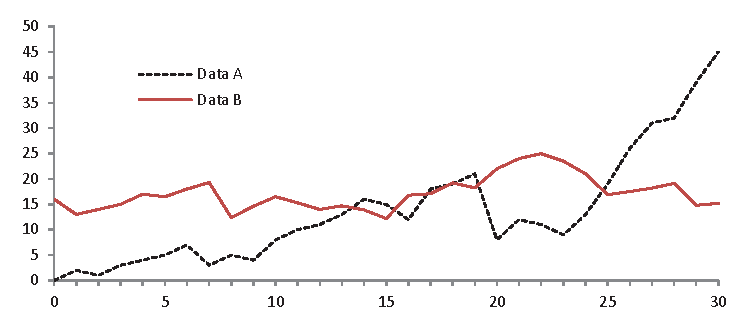
\includegraphics[width=\textwidth]{fig1.eps}
\caption{A figure caption is always placed below the illustration.
Please note that short captions are centered, while long ones are
justified by the macro package automatically.} \label{fig1}
\end{figure}

\begin{theorem}
This is a sample theorem. The run-in heading is set in bold, while
the following text appears in italics. Definitions, lemmas,
propositions, and corollaries are styled the same way.
\end{theorem}
%
% the environments 'definition', 'lemma', 'proposition', 'corollary',
% 'remark', and 'example' are defined in the LLNCS documentclass as well.
%
\begin{proof}
Proofs, examples, and remarks have the initial word in italics,
while the following text appears in normal font.
\end{proof}
For citations of references, we prefer the use of square brackets
and consecutive numbers. Citations using labels or the author/year
convention are also acceptable. The following bibliography provides
a sample reference list with entries for journal
articles~\cite{ref_article1}, an LNCS chapter~\cite{ref_lncs1}, a
book~\cite{ref_book1}, proceedings without editors~\cite{ref_proc1},
and a homepage~\cite{ref_url1}. Multiple citations are grouped
\cite{ref_article1,ref_lncs1,ref_book1},
\cite{ref_article1,ref_book1,ref_proc1,ref_url1}.
%
% ---- Bibliography ----
%
% BibTeX users should specify bibliography style 'splncs04'.
% References will then be sorted and formatted in the correct style.
%
% \bibliographystyle{splncs04}
% \bibliography{mybibliography}
%
\begin{thebibliography}{8}
\bibitem{ref_article1}
Author, F.: Article title. Journal \textbf{2}(5), 99--110 (2016)

\bibitem{ref_lncs1}
Author, F., Author, S.: Title of a proceedings paper. In: Editor,
F., Editor, S. (eds.) CONFERENCE 2016, LNCS, vol. 9999, pp. 1--13.
Springer, Heidelberg (2016). \doi{10.10007/1234567890}

\bibitem{ref_book1}
Author, F., Author, S., Author, T.: Book title. 2nd edn. Publisher,
Location (1999)

\bibitem{ref_proc1}
Author, A.-B.: Contribution title. In: 9th International Proceedings
on Proceedings, pp. 1--2. Publisher, Location (2010)

\bibitem{ref_url1}
LNCS Homepage, \url{http://www.springer.com/lncs}. Last accessed 4
Oct 2017
\end{thebibliography}
\end{document}
